%In this section, the layer is described in some detail in terms of its specific subsystems. Describe each of the layers and its subsystems in a separate chapter/major subsection of this document. The content of each subsystem description should be similar. Include in this section any special considerations and/or trade-offs considered for the approach you have chosen.%
This section discusses the software layer which consists of three major subsystems. 

\begin{figure}[h!]
	\centering
 	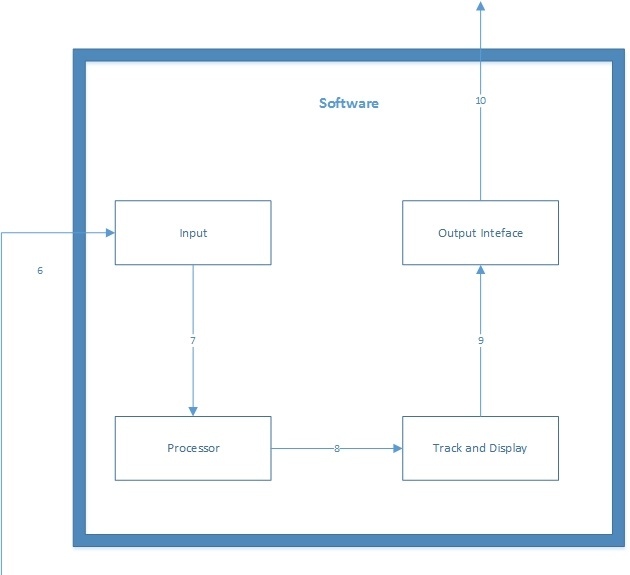
\includegraphics[width=0.60\textwidth]{images/Software.jpg}
 \caption{Software Subsystem}
\end{figure}

\subsection{Input Subsystem}
%This section should be a general description of a particular subsystem for the given layer. For most subsystems, an extract of the architectural block diagram with data flows is useful. This should consist of the subsystem being described and those subsystems with which it communicates.
The input subsystem is responsbile for receiving video input and sending it to the processing subsystem.

\begin{figure}[h!]
	\centering
 	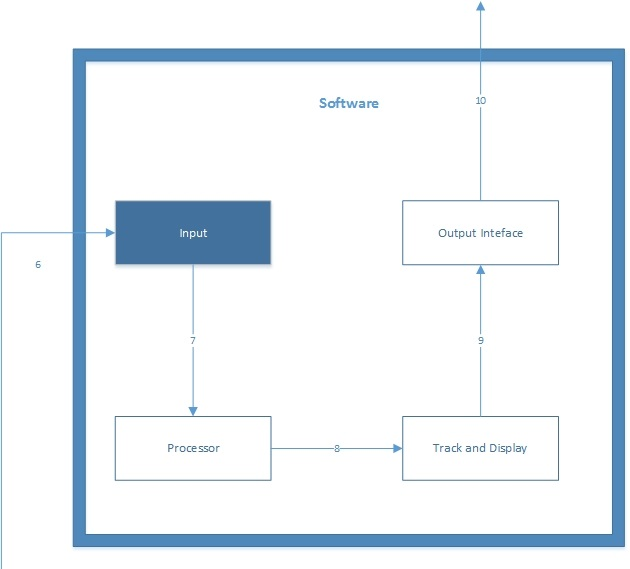
\includegraphics[width=0.60\textwidth]{images/Software_Input.jpg}
 \caption{Input Subsystem}
\end{figure}

\subsubsection{Assumptions}
%Any assumptions made in the definition of the subsystem should be listed and described. Pay particular attention to assumptions concerning interfaces and interactions with other layers.
We are assuming that we are getting the required video data from the Cypress CX3 or any other USB device. The software is flexible enough to be able to read the data from a file or directly from the hardware. 


\subsubsection{Responsibilities}
%Each of the responsibilities/features/functions/services of the subsystem as identified in the architectural summary must be expanded to more detailed responsibilities. These responsibilities form the basis for the identification of the finer-grained responsibilities of the layer's internal subsystems. Clearly describe what each subsystem does.
This subsystem is responsible for properly receiving the video data and sending it to the processor subsystem. 

\subsubsection{Subsystem Interfaces}
%Each of the inputs and outputs for the subsystem are defined here. Create a table with an entry for each labelled interface that connects to this subsystem. For each entry, describe any incoming and outgoing data elements will pass through this interface.
The input could either from a file (for test purposes) or a live stream from the cypress camera. The details are shown in the table. 


\begin {table}[H]
\caption {Input Subsystem interface} 
\begin{center}
    \begin{tabular}{ | p{1cm} | p{6cm} | p{3cm} | p{3cm} |}
    \hline
    ID & Description & Inputs & Outputs \\ \hline
    \#06 & Receive video data & \pbox{3cm}{From Camera} & \pbox{3cm}{ Video data  }  \\ \hline
    %\#02 & Input video data from the File & \pbox{3cm}{N/A} & \pbox{3cm}{Video data}  \\ \hline
    \end{tabular}
\end{center}
\end{table}

\subsection{Processor Subsystem}
The processor subsystem takes in the video input, processes it sends the processed data to the Track and Display subsystem.

\begin{figure}[h!]
	\centering
 	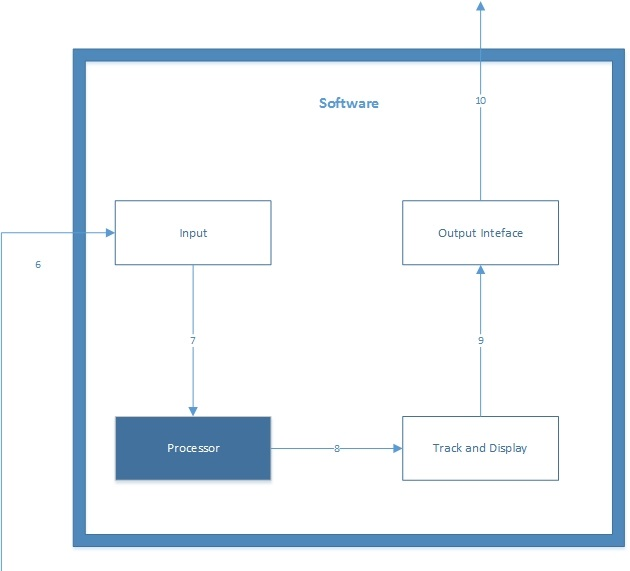
\includegraphics[width=0.60\textwidth]{images/Software_Processor.jpg}
 \caption{Processor Subsystem}
\end{figure}



\subsubsection{Assumptions}
%Any assumptions made in the definition of the subsystem should be listed and described. Pay particular attention to assumptions concerning interfaces and interactions with other layers.
We assume that we are getting video data from the Input Subsystem at 30 frames per second. 

%Repeat for each subsystem
\subsubsection{Responsibilities}
%Each of the responsibilities/features/functions/services of the subsystem as identified in the architectural summary must be expanded to more detailed responsibilities. These responsibilities form the basis for the identification of the finer-grained responsibilities of the layer's internal subsystems. Clearly describe what each subsystem does.
The processor is responsible for utilizing various computer vision algorithms to properly track the pupil. First, the processor needs to smooth each frame in the video. Next, it needs to apply the canny edge detector
to detect all the edges. Finally, this processor sends all the detected edges to the Track and Display subsystem. 

\subsubsection{Subsystem Interfaces}
%Each of the inputs and outputs for the subsystem are defined here. Create a table with an entry for each labelled interface that connects to this subsystem. For each entry, describe any incoming and outgoing data elements will pass through this interface.
This subsystem gets input of video data and output of a somewhat refined video data.

\begin {table}[H]
\caption {Processor Subsystem interface} 
\begin{center}
    \begin{tabular}{ | p{1cm} | p{6cm} | p{3cm} | p{3cm} |}
    \hline
    ID & Description & Inputs & Outputs \\ \hline
    \#07 & Process Video Frames & \pbox{3cm}{Video Data} & \pbox{3cm}{ Detected Edges }  \\ \hline
    %\#xx & Description of the interface/bus & \pbox{3cm}{N/A} & \pbox{3cm}{output 1}  \\ \hline
    \end{tabular}
\end{center}
\end{table}

\subsection{Track and Display Subsystem}
This subsystem receives some video data whose edges have been detected by the processor subsytem and it tracks and displays the results. 

\begin{figure}[h!]
	\centering
 	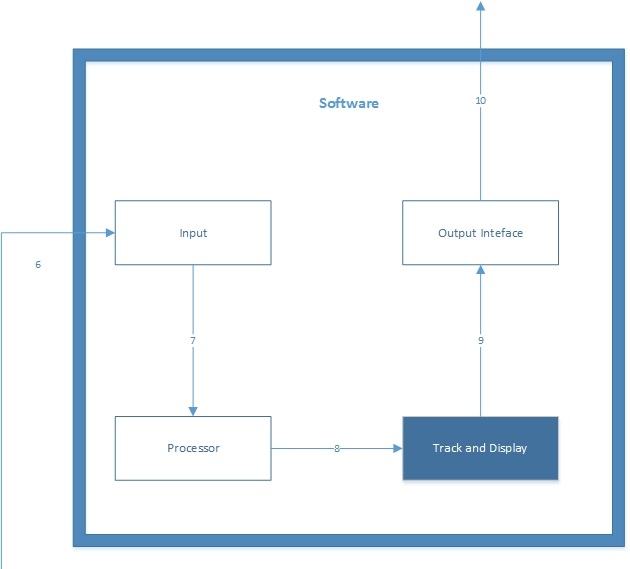
\includegraphics[width=0.60\textwidth]{images/Software_Track.jpg}
 \caption{Tracker Subsystem}
\end{figure}

\subsubsection{Assumptions}
%Any assumptions made in the definition of the subsystem should be listed and described. Pay particular attention to assumptions concerning interfaces and interactions with other layers.
We assume that this subsystem recieves frames whos edges have been detected. 

%Repeat for each subsystem
\subsubsection{Responsibilities}
%Each of the responsibilities/features/functions/services of the subsystem as identified in the architectural summary must be expanded to more detailed responsibilities. These responsibilities form the basis for the identification of the finer-grained responsibilities of the layer's internal subsystems. Clearly describe what each subsystem does.
This subsystem is responsible for applying the pupil tracking algorithm to the input it receives. It then applies the RANSAC algorithm to fit an ellipse to the pupil. Finally, it
displays the video with tracked pupil. 

\subsubsection{Subsystem Interfaces}
%Each of the inputs and outputs for the subsystem are defined here. Create a table with an entry for each labelled interface that connects to this subsystem. For each entry, describe any incoming and outgoing data elements will pass through this interface.
This subsystem receives edges that were detected by the processing subsystem and outputs the final results in a video stream. 

\begin {table}[H]
\caption {Track and Display Subsystem interface} 
\begin{center}
    \begin{tabular}{ | p{1cm} | p{6cm} | p{3cm} | p{3cm} |}
    \hline
    ID & Description & Inputs & Outputs \\ \hline
    \#08 & Receive data and display & \pbox{3cm}{Detected Edges } & \pbox{3cm}{Tracked Eye}  \\ \hline
    %\#xx & Description of the interface/bus & \pbox{3cm}{N/A} & \pbox{3cm}{output 1}  \\ \hline
    \end{tabular}
\end{center}
\end{table}


\subsection{Output Subsystem}
This subsystem simply provides an interface to send a video stream to some external device or module via ethernet or USB. The exeternal device or module shall be either a computer monitor or a cell phone or a webpage. 


\begin{figure}[h!]
	\centering
 	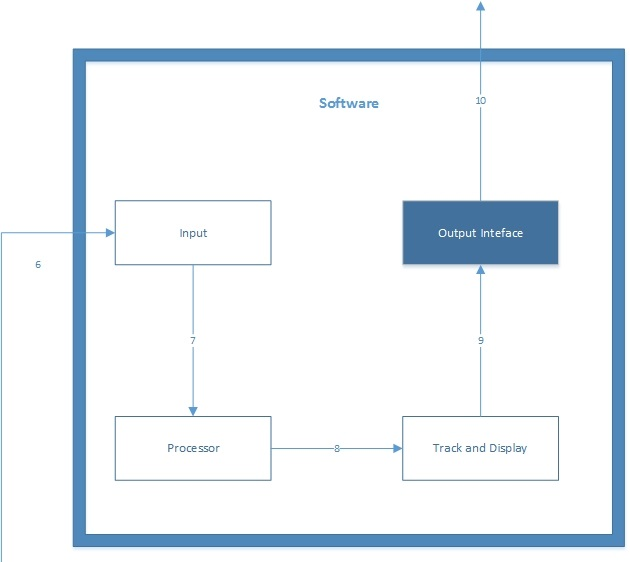
\includegraphics[width=0.60\textwidth]{images/Software_Output.jpg}
 \caption{Output Subsystem}
\end{figure}

\subsubsection{Assumptions}
%Any assumptions made in the definition of the subsystem should be listed and described. Pay particular attention to assumptions concerning interfaces and interactions with other layers.
We assume that this subsystem recieves video frames that show the tracked pupil. 

%Repeat for each subsystem
\subsubsection{Responsibilities}
%Each of the responsibilities/features/functions/services of the subsystem as identified in the architectural summary must be expanded to more detailed responsibilities. These responsibilities form the basis for the identification of the finer-grained responsibilities of the layer's internal subsystems. Clearly describe what each subsystem does.
This subsystem is responsible for properly sending the final result (video) of the entire system to an output device such a computer monitor. 

\subsubsection{Subsystem Interfaces}
%Each of the inputs and outputs for the subsystem are defined here. Create a table with an entry for each labelled interface that connects to this subsystem. For each entry, describe any incoming and outgoing data elements will pass through this interface.
This subsystem receives videos and provides an interface for an output device such as a monitor.  

\begin {table}[H]
\caption {Output Subsystem interface} 
\begin{center}
    \begin{tabular}{ | p{1cm} | p{6cm} | p{3cm} | p{3cm} |}
    \hline
    ID & Description & Inputs & Outputs \\ \hline
    \#09 & Send video data to external device & \pbox{3cm}{Tracked Eye } & \pbox{3cm}{Tracked Eye}  \\ \hline
    %\#xx & Description of the interface/bus & \pbox{3cm}{N/A} & \pbox{3cm}{output 1}  \\ \hline
    \end{tabular}
\end{center}
\end{table}



